\documentclass[aspectratio=169]{beamer}

\usetheme{metropolis}
\usepackage{appendixnumberbeamer}

\usepackage{booktabs}
\usepackage[scale=2]{ccicons}

\usepackage{pgfplots}

\usepackage{xspace}
\newcommand{\themename}{\textbf{\textsc{metropolis}}\xspace}

\usepackage[utf8]{inputenc}
\usepackage[T1]{fontenc}

\usepackage{listings}
\usepackage{xcolor, colortbl}
\usepackage{multicol}
\usepackage{chronology}

\definecolor{done}{rgb}{0.36, 0.72, 0.36}
\definecolor{doing}{rgb}{1.0, 0.8, 0.0}
\definecolor{scheduled}{rgb}{0.25, 0.54, 0.79}

\newcommand{\done}{\cellcolor{done}}
\newcommand{\scheduled}{\cellcolor{scheduled}}
\newcommand{\doing}{\cellcolor{doing}}

\bibliographystyle{unsrt}

\lstdefinestyle{sharpc}{language=[Sharp]C, frame=lr, rulecolor=\color{blue!80!black}}


\title{Eliminando Gargalos de Processamento \newline Utilizando Rust}
\date{}
\author{Johnathan Fercher}
%\institute{Braspag}
\titlegraphic{\hfill
\includegraphics[height=2.0cm]{imgs/logo.png}}

\begin{document}
\maketitle

\begin{frame}{Sumário}
  \setbeamertemplate{section in toc}[sections numbered]
  \tableofcontents[hideallsubsections]
\end{frame}

\section{Introdução}
\begin{frame}{Introdução}
	\begin{center}
		
\includegraphics[width=2.5cm]{imgs/rust.png}
	\end{center}

	Uma linguagem de programação de sistemas que roda incrivelmente rápido, previne falhas de segmentação, e garente segurança entre threads.
\end{frame}

\begin{frame}{Motivação}
	\begin{quote}
		\hspace{0.5cm}"O poder de processamento dobra a cada 18 meses."
		
		\hspace{8.2cm}Lei de Moore, 1965.
	\end{quote}
\end{frame}

\begin{frame}{Motivação}
	\begin{center}
		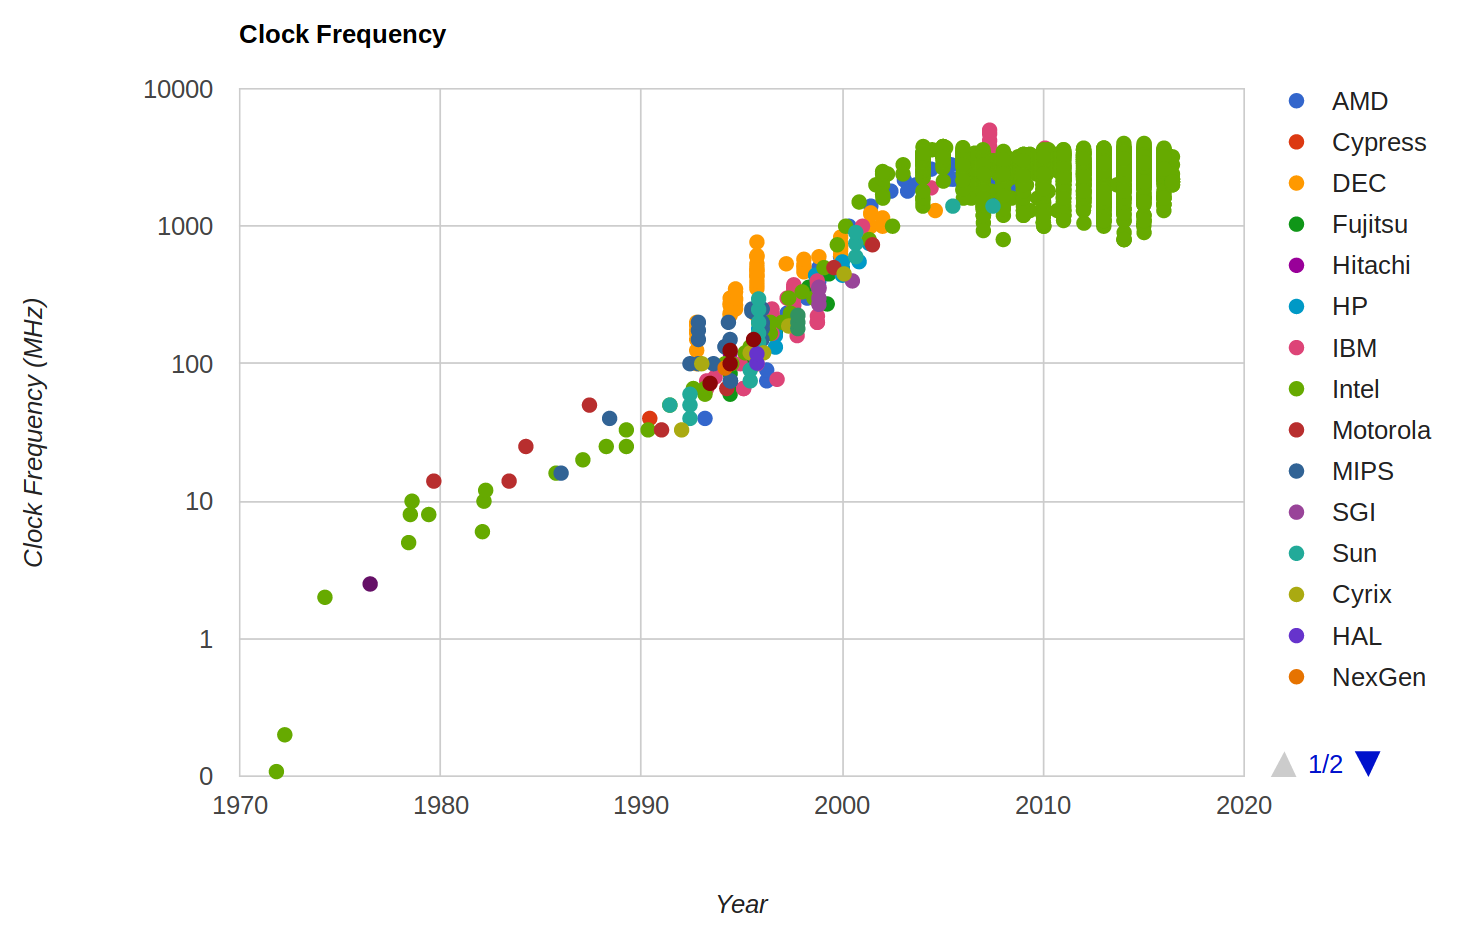
\includegraphics[width=12cm]{imgs/clock-rate-history.png}
	\end{center}
\end{frame}

\begin{frame}{Motivação}
	\begin{center}
		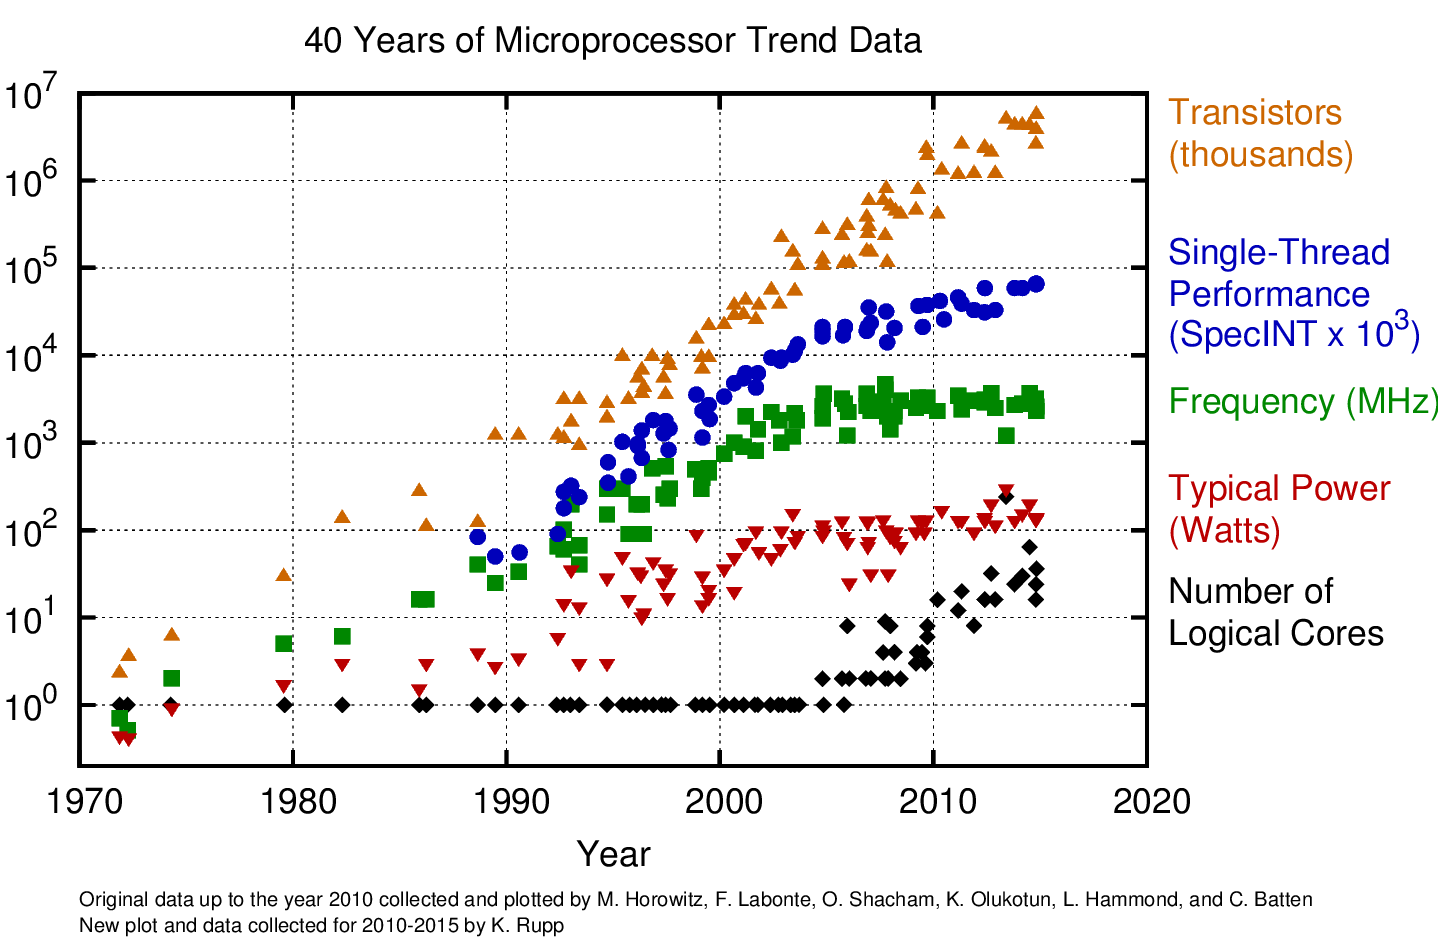
\includegraphics[width=12.5cm]{imgs/cores-history.png}
	\end{center}
\end{frame}

\begin{frame}{Motivação}
	\begin{quote}
		"The way the processor industry is going, is to add more and more cores, but nobody knows how to program those things. I mean, two, yeah; four, not really; eight, forget it."
		
		\hspace{8.2cm}Steve Jobs, Apple.
	\end{quote}
\end{frame}

\begin{frame}{História}
	\begin{chronology}[5]{2002}{2015}{80ex}[\textwidth]
		\event[2002]{2003}{C \& LLVM}
		\event{2006}{Graydon Hoare}
		\event{2009}{Mozilla}
		\event{2010}{Rust-c in Rust}
		\event{2011}{Rust-c using LLVM}
		\event{2012}{Alpha}
		\event{2013}{Cargo}
		\event{2015}{Stable}
	\end{chronology}
\end{frame}

\begin{frame}{Desenvolvimento}
	\begin{itemize}
		\item Licensa MIT no Github;
		\item Duas versões: Stable e Nightly;
		\item Processo de RFC;
		\item Quando uma RFC é aprovada ela é adicionada na versão Nightly;
		\item Após algum tempo em Nightly, ela pode ser adicionada na versão Stable, deixada de lado ou alterada;	
	\end{itemize}
\end{frame}

\section{Quem usa? E para que?}

\begin{frame}{Quem usa? E para que?}
	\begin{center}
		
\includegraphics[width=4.5cm]{imgs/dropbox.png}	
		
		"Optimizing cloud file-storage."
	\end{center}
\end{frame}

\begin{frame}{Quem usa? E para que?}
	\begin{center}
		
\includegraphics[width=4.5cm]{imgs/canonical.jpeg}	
		
		"Everything from server monitoring to middleware!"
	\end{center}
\end{frame}

\begin{frame}{Quem usa? E para que?}
	\begin{center}
		
\includegraphics[width=4.5cm]{imgs/smartthings.png}	
		
		"Developing memory-safe embedded applications on our SmartThings Hub and supporting services in the cloud."
	\end{center}
\end{frame}

\begin{frame}{Quem usa? E para que?}
	\begin{center}
		
\includegraphics[width=4.5cm]{imgs/mozilla.png}	
		
		"Building the Servo browser engine, integrating into Firefox, other projects."
	\end{center}
\end{frame}

\begin{frame}{Quem usa? E para que?}
	\begin{center}
		
\includegraphics[width=4.5cm]{imgs/coursera.png}	
		
		"Programming Assignments in secured Docker containers."
	\end{center}
\end{frame}

\begin{frame}{Quem usa? E para que?}
	\begin{center}
		
\includegraphics[width=2.2cm]{imgs/chef.png}	
		
		"Letting you develop, deploy and manage infrastructure, run-time environments and applications."
	\end{center}
\end{frame}

\begin{frame}{Quem usa? E para que?}
	\begin{center}
		
\includegraphics[width=4.5cm]{imgs/atlassian.png}	
		
		"We use Rust in a service for analyzing petabytes of source code."
	\end{center}
\end{frame}

\begin{frame}{Quem usa? E para que?}
	\begin{center}
		
\includegraphics[width=3.0cm]{imgs/npm.jpeg}	
		
		"Replacing C and rewriting performance-critical bottlenecks in the registry service architecture."
	\end{center}
\end{frame}

\begin{frame}{Quem usa? E para que?}
	\begin{center}
		
\includegraphics[width=3.5cm]{imgs/habitat.png}	
		
		"Habitat is automation that travels with the app. Rust aid us to remove bottlenecks."
	\end{center}
\end{frame}

\begin{frame}{Quem usa? E para que?}
	\begin{itemize}
		\item No site oficial da linguagem há mais 123 empresas que deixaram claro que utilizam Rust;
	\end{itemize}
\end{frame}

\section{Hands-On Rust}

\begin{frame}{Sistema de contagem de votos}
	Voto: 
	\begin{itemize}
		\item Number: Option<u8>;
		\item Age: u8;
		\item State: state\_type;
		\item Gender: gender\_type;
	\end{itemize}
\end{frame}

\begin{frame}{Sistema de contagem de votos}
	\begin{enumerate}
		\item Criar um projeto utilizando cargo;
		\item Instalar o crate (votes\_generator) do github;
		\item Criar uma classe que remove dados duplicados;
		\item Criar uma classe que computa o vencedor;
		\begin{enumerate}
			\item For loop;
			\item Filter;
		\end{enumerate}
		\item Instalar o crate (group\_by) do cargo;
		\item Criar um método que computa o vencedor com agrupamento;
	\end{enumerate}
\end{frame}

\section{Material de estudo}

\begin{frame}{Rust by Example}
	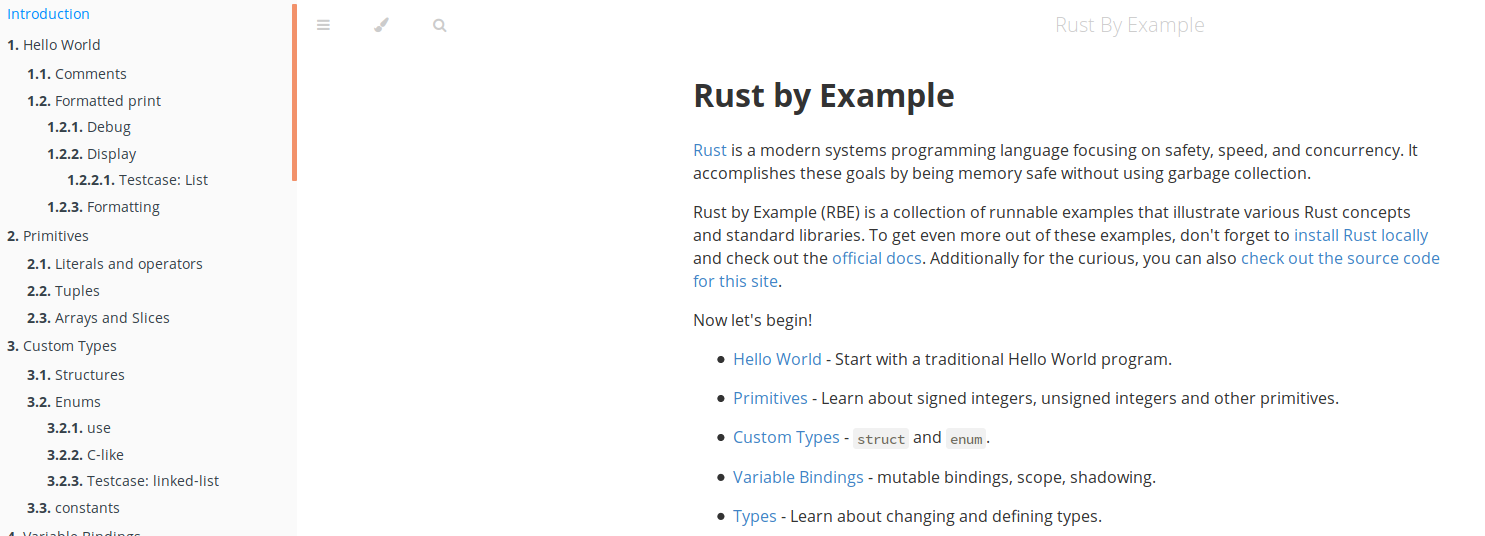
\includegraphics[width=15.0cm]{imgs/rust-by-example.png}	
\end{frame}

\begin{frame}{Rust - Concorrência e alta performance com segurança}
	\begin{center}
		
\includegraphics[width=5.0cm]{imgs/casa-do-codigo-rust.jpg}	
	\end{center}
\end{frame}

\begin{frame}{Programming Rust}
	\begin{center}
		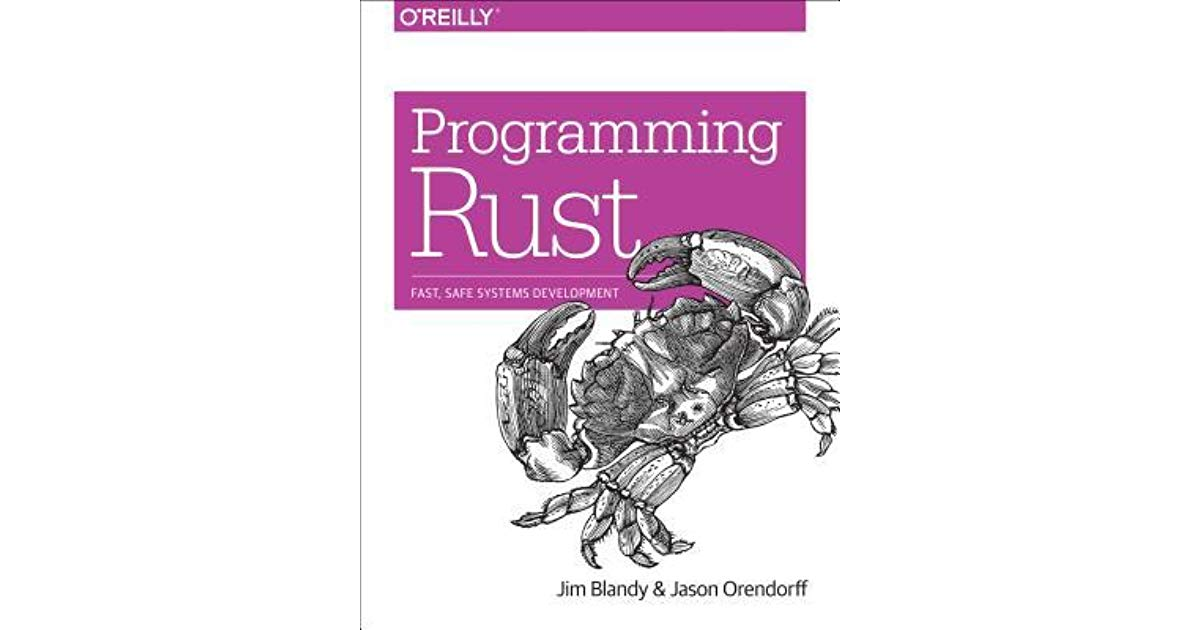
\includegraphics[width=13.0cm]{imgs/programming-rust.jpg}	
	\end{center}
\end{frame}

\begin{frame}{Programming Rust}
	\begin{center}
		
\includegraphics[width=5.0cm]{imgs/hands-on-functional-programming-in-rust.jpg}	
	\end{center}
\end{frame}

\begin{frame}[standout]
  Obrigado
\end{frame}

\end{document}
